\documentclass[lnbip]{svmultln}

\usepackage{makeidx}
\usepackage{graphicx}
\usepackage{url}

\begin{document}

\mainmatter

\title{Open Source and Agile Methods:\\Two worlds closer than it
  seems}

\titlerunning{Open Source and Agile Methods}

\author{Hugo Corbucci\inst{1} and Alfredo Goldman\inst{1}}

\authorrunning{Hugo Corbucci et al.}

\tocauthor{Hugo Corbucci, Alfredo Goldman}

\institute{Instituto de Matem\'{a}tica e Estat\'{i}stica (IME)\\
  Universidade de S\~{a}o Paulo (USP) - Brazil\\
  \email{corbucci@ime.usp.br} and \email{gold@ime.usp.br} }
 
\maketitle

\begin{abstract}
  Agile methods and open source software communities have different
  approaches to produce high quality and successful software. However
  agile methodologies are not very diffused in open source communities
  nor the members of those communities follow many agile
  practices.

% TODO Mais abstract

  \keywords{agile software development, open source software,
    distributed agile, }
\end{abstract}

\section{Introduction}

Typical Open Source (OS) projects (the scope of of OS project will be
narrowed according to Section \ref{sec:scope}) usually receive
the collaboration of many geographically distant people
\cite{report:dempsey1999}. At first glance, this argument could
indicate that such projects are not candidates for the use of agile
methods since some basic values seem to be missing. In this case, the
distance and diversity separating developers deteriorates
communication, a very important value within agile methods. However,
it is common to identify some principles presented by the agile
manifesto \cite{url:agilemanifesto} on many open source software
projects. Being ready for changes, working with continuous feedback,
delivering real features, respecting collaborators and users and
facing challenges are expected attitudes from agile developers
naturally found in the Free and Open Source Software (FOSS)
communities\cite{gabriel2005}.

During a workshop \cite{conference:oopsla2007} held at OOPSLA 2007
celebrating 20 years from the publication of ``No Silver Bullets''
\cite{brooks1987}, agile methods and OS software development were
mentioned as two failed silver bullets having both brought great
benefit to the software community. During the same workshop the
question was raised whether the use of several failed silver bullets
simultaneously could not raise production levels by an order of
magnitude. This work is an attempt to suggest one of those merges to
partially tackle software development problems.

% TODO Write the agenda

\section{Scopes}
\label{sec:scope}

The FOSS environment as well as the agile both comprehend such a wide
variety of projects, people and contexts that it is very hard to cover
all of them. Therefore it is necessary to first define which part of
each community will be analysed in this work.
\\

Throughout this work, any software engineering method that follows the
principles of the agile manifesto \cite{url:agilemanifesto} will be
considered and treated as an agile method. Focus will be given on the
most known methods, such as eXtreme Programming (XP) \cite{XP2002},
Scrum \cite{schwaber2004} and the Crystal family
\cite{cockburn2002}. Closely related ideas will also be mentioned from
the wider Lean philosophy \cite{ohno1998} and its application to
software development \cite{poppendieck2005}.
\\

The terms ``open source software'' and ``free software'' will be
considered the same in this work although they have some differences
in their specific contexts \cite[Ch. 1, Free Versus Open
source]{fogel2005}. Projects will be called to be open source (or
free) if their source code is available and modifiable by anyone with
the required technical knowledge, without prior consent from the
original author and without any charge.

OS projects essentially controlled by a single company fall out of the
scope of this work. The reason for such reduction of scope is that
projects controlled by companies, whether they have a public source
code and accept external collaboration or not, can be run with any
software engineering method established in the company since it can be
enforced to the employees of this company.

Considering this scope, it is important to characterize the people
involved in such kind of projects. In 2002, the FLOSS Project
\cite{url:flossproject} published a report about a survey they
conducted regarding FOSS contributors. Their collected data
\cite{url:flossdata} shows that 78.77\% of the contributors are
employed or self-employed (question 42) and that only 50.82\% of the
OS community are software developers while 24.76\% do not earn their
main income with software development (question 10).  In addition to
those results, the survey presents the fact that 78.78\% of the
collaborators consider their OS tasks more joyful (question 22.2) than
their regular activities and 42.3\% also consider them better
organized (question 22.4). As an outcome of those results, we could
say that OS contributors perceive their activities both pleasurable
and effective.

% TODO Rever essas porcentagem para trocar por algo mais interessante

Another survey \cite{reis2003} points out that 74\% of open source
projects have teams with up to 5 people and 62\% of the contributors
work with each other over the Internet and have never met physically.

Considering such characterization of the FOSS community, the next
section presents what is the relation between such development
environment with the ideas and guidelines of agile methodologies.

\section{How closely related are Open source and Agile?}
\label{sec:relation}

In Martin Fowler's first version of ``The New Methodology''
\cite{url:fowler2000orig}, he included open source software
development as part of the new methodology of software development
along with now well known Agile methods. He decided to remove it from
the final article because the FOSS environment is so big and spread
that any attempt to characterize the development process would
undoubtedly fail on a given environment.

Afterwards, in 2002, Warsta \cite{warsta2002} published a review about
agile software development methods including and discussing OSS as an
agile method.  However, he stresses that FOSS development is not a
precise method and evolves differently for each project. Indeed, Eric
Raymond's description of the development process from ``The Cathedral
and the Bazaar'' \cite{raymond1999} is closer to an experience report
than to the description of a process with guidelines and
practices. Nevertheless, Raymond's text presents several actions that
could be related to the agile manifesto \cite{url:agilemanifesto} and
are common in other FOSS projects.

FOSS communities are, by definition, a group of people gathered around
a FOSS project. A working and useful software project attracts
individuals to collaborate to evolve the
software\cite{crowston2002}. It is the people's interactions that will
define the development process, tools and even the goals of the
software. FOSS projects that do not evolve to fit the needs of its
community are abandoned in a highly competitive environment where the
best (in certain criteria) gains adopters in a thin line between
success and oblivion.

From such aspects, FOSS project share a lot in common with the values
presented by agile methods. The practices are also quite similar. Eric
Raymond quotes Linus Torvalds about two specific development policy
for the Linux Kernel.
\begin{enumerate}
\item[7.] Release early. Release often. And listen to your customers.
\item[8.] Given a large enough beta-tester and co-developer base,
  almost every problem will be characterized quickly and the fix will
  be obvious to someone.
\end{enumerate}

The first policy hints for an iterative and short development process
with frequent feedback input. The second one points to a large amount
of test done frequently. Those ideas are core principles for agile
methods and largely applied to several successful FOSS projects.
% TODO Referencias

We can, therefore, state that the FOSS community have a culture that
is similar to the one of the agile community. Given that there is such
proximity between agile methods and FOSS development, it must not be
forgotten that the environments in which each solution out stands are
quite different.

Open source software is stronger when it comes to products that
``scratch a developer's itch'' \cite{fitzgerald2000}, i.e. a product
in which the own developer can be the user. Such product evolve across
the Internet gathering volunteers interested in such development by
releasing versions of the software frequently.

Agile methods come from industry consultants with focus on business
problems and customer satisfaction through frequent high quality
releases. To achieve such goal, an ideal agile team needs motivated
competent people closely gathered with freedom to improve their
environment and process to enable what Cockburn calls osmotic
communication \cite{cockburn2004}.

The most critical discrepancy is the one regarding
communication. Agile methods stress out that many software development
problems come from the lack of high quality communication and the best
way to mitigate it is to keep people close and in constant
contact. Open source software are inherently distributed and
frequently run by people that only meet through the Internet. Could
there be a way to unite the strength of both communities and improve
development in distributed environments with changing requirements?

In order to evaluate this possibility, we decided to elaborate two
surveys. The next section describes how the surveys were elaborated
and what information were expected to be collected.

\section{Surveys}
\label{sec:surveys}

Since the motivation to write was to understand if the agile community
and the FOSS community could share more principles and practices, one
survey was directed to agile practitioners while the other was aimed to
FOSS contributors.  Each survey intended to characterize the answering
public, was available on the Internet and was spread in channels
common to the target communities.

The next subsection presents the survey created for the FLOSS
community while the following one shows the one aimed to the agile
community.

\subsection{To the FLOSS community}
\label{subsec:floss-survey}

For both surveys, part of the goal was to identify which part of the
community answered the question and how representatives they were for
their community. Therefore, the first set of questions were pretty
similar between both surveys and inquired the participants about their
year of birth and country of residence. Both surveys also tried to
evaluate the experience of the participants in their community. For
the FLOSS community that translated to the amount of project with
which the participant had contributed with as well the first year of
contribution.

This last question as well as the following ones were only displayed
if the participant had contributed to at least one FLOSS project since
most questions would be meaningless otherwise. In order to narrow the
environment that the participants would have to evaluate as well as
their experience in such project, they were asked the name of the main
project as well as their role in the project.

To understand how the project ensure communication between its
collaborators, the participants were asked how big was the project
team and, if there was a team (not a single person team) what was the
communication channel used to communicate among them. The survey also
asked the participant to evaluate the quality of the communication
through that channel. The survey also included a similar question
regarding the communication channel with the users of project and its
evaluated quality.

At last, the survey inquired the participants about which of 8 tools
did the project already used and how they would classify the
usefulness of those tools to mitigate their problem with the project's
development.

A paper version of the survey can be found in Appendix
\ref{appendix:a}\footnote{The online address of the survey was omitted
  according to the submission rules}.
% while the online version can be accessed at {\tt
%   http://www.ime.usp.br/~corbucci/floss-survey}.
The survey was announced via twitter\footnote{http://twitter.com} by
the authors and received the support of
GitHub\footnote{http://github.com} who asked their users to fill in
the survey.

The survey was also sent to other FLOSS project hosting systems such
as SourceForge.net, LaunchPad.net, CodeHaus, Google Code but none
answered the request or provided any sort of answers.  It was also
published in a few blogs related to the FLOSS community and mailing
lists for the Python community as well other international mailing
lists.

\subsection{To the Agile community}
\label{subsec:agile-survey}

The beginning of the survey directed to the Agile community was very
similar to the one to the FLOSS community since its goal was to
collect data to characterize the participants.  After the first
questions regarding the residence country and the year of bird, the
agile survey inquired the participants about their agile experience
asking on how many agile projects they participated in and when was
their first agile project.

Similarly to the FLOSS survey, this last question as well as the
following were only displayed to participants that had been in at
least one of agile project. The survey kept on asking about the
participant's main role in the project and the size of the team
involved. The participant was then asked to inform the main
communication channel used to communicate with the client of that
project as well as the quality of communication on that channel.

Divergence from the FLOSS survey followed with a question inquiring if
the participant had any previous experience with applying agile
methods in a distributed environment. If so, the participant was asked
to describe the communication channel used in this distributed project
and its quality.

The participants were then asked to sort the 3 most critical problems
encountered in the agile environment in which they
participated. Afterwards the participant should sort the top 3 tools
(out of 8) that would help in a distributed agile environment.

Finally, the participants were asked if they were FLOSS contributors
and, if so, how agile they considered their FLOSS project and how
would they sort the problems and tools in that FLOSS environment.

The paper version of this version can be found in Appendix
\ref{appendix:b}\footnote{The online address of the survey was omitted
  according to the submission rules}
% while the online version can be found at {\tt
%   http://www.ime.usp.br/~corbucci/agile-survey}.
This survey was announced in mailing lists related to the subject as
well as blogs and twitter by various supporters. The authors also
sought the support from the Agile Alliance but no answer was provided.

\section{Survey results}
\label{sec:results}

The surveys were ellaborated to be answered by the participants
through the Internet and used some dynamic contents to minimize the
amount of answers each participants should provide. Such work was
performed through Javascript but was not validated against older
browsers such as Internet Explorer 6 and 7. Trying to answer the
surveys using those browsers resulted in an invalid answer. This
unexpected error provided an extra information regarding the browser
used by each community.

The individual results of each survey provide interesting data by
themselves and are described in subsections \ref{subsec:floss-results}
and \ref{subsec:agile-results} for the FLOSS survey and the agile one
respectively.

\subsection{Individual results from the FLOSS community}
\label{subsec:floss-results}

The results for the FLOSS survey were collected between 2009/07/28 and
2009/11/01. The survey received 309 entries from which 3 were
duplicated data (same IP address and time entry) while 4 others were
invalid answers (caused by Javascript errors). This unexpected data
shows that approximately 1\% of people who are connected with FLOSS
communities use a browser not compatible with the standards.

Out of those 302 valid entries, 122 were answers in which the
participant never contributed to a FLOSS project but considered
herself as part of the FLOSS community. So only about 60\% of the
FLOSS community actually contributes with projects.

\begin{figure}[htb]
  \begin{minipage}[t]{0.5\linewidth}
    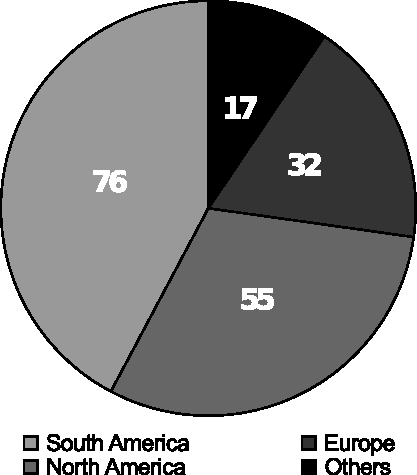
\includegraphics[scale=0.8]{floss-world.pdf}
    \caption{FLOSS answers in the world}
    \label{fig:floss-world}
  \end{minipage}
  \begin{minipage}[t]{0.5\linewidth}
    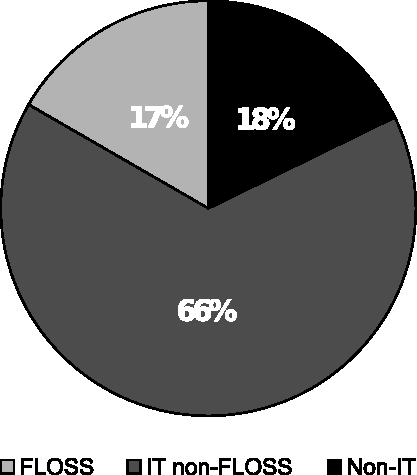
\includegraphics[scale=0.8]{floss-income.pdf}
    \caption{Main income origin for FLOSS participants}
    \label{fig:floss-income}
  \end{minipage}
\end{figure}

The analysis was performed over the 180 answers left since they
provided more interesting data. Figure \ref{fig:floss-world}
represents the distribution of the answers around the globe. Figure
\ref{fig:floss-income} shows the main income origin of the
participants. The average age of the participants was 28 years old and
the average year of for the first FLOSS contribution was 2003. Figure
\ref{fig:floss-firstxp} shows that younger participants started
contributing earlier in their life than older participants which can
be explained by the increasing ease to get in touch with a computer in
the last years.

\begin{figure}[htb]
  \centering
  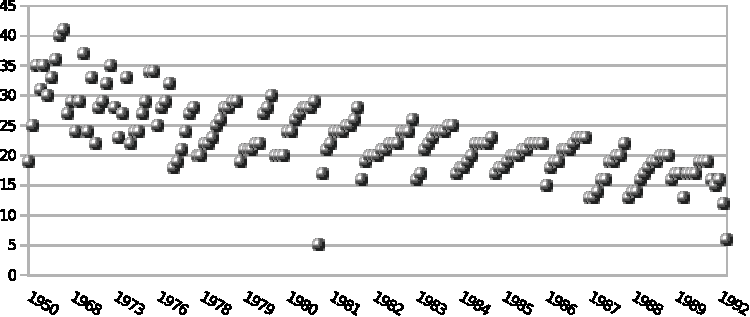
\includegraphics[scale=.9]{floss-firstxp.pdf}
  \caption{Age of first FLOSS contribution by year of birth}
  \label{fig:floss-firstxp}
\end{figure}
% TODO Melhorar gráfico de idades de contribuição inicial

About two thirds of the participants were project maintainers,
commiters or programmers. The last third was partitioned between other
roles as shows Figure \ref{fig:floss-roles}. Team sizes were also
fairly representative since only 6\% of the project were single person
team while 48\% were up to 5 team members. Figure
\ref{fig:floss-teams} shows those results and the reported team
sizes. It is interesting to notice that such profile is similar to the
one described by Reis \cite{reis2003} obtained in 2003.

\begin{figure}[htb]
  \begin{minipage}[t]{0.5\linewidth}
    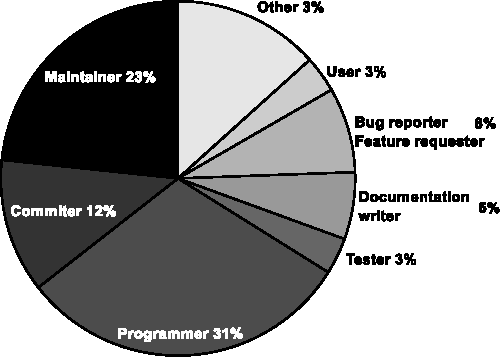
\includegraphics[scale=0.8]{floss-roles.pdf}
    \caption{Distribution of participant's roles}
    \label{fig:floss-roles}
  \end{minipage}
  \begin{minipage}[t]{0.5\linewidth}
    \begin{flushright}
      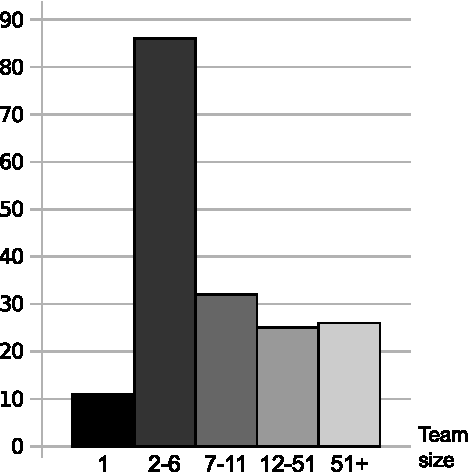
\includegraphics[scale=0.65]{floss-teams.pdf}
      \caption{FLOSS projects reported team sizes}
      \label{fig:floss-teams}
    \end{flushright}
  \end{minipage}
\end{figure}

Regarding the main communication channels, it seems to have changed a
little since the FLOSS world research or Reis' one. The main
communication channels with the rest of the team are still mailing
lists (27\%) and Internet Relay Chat (IRC - 23\%). However the amount
of people using face to face communication within the team shows some
increase (now at 15\%). The quality of the communication in those
channels was fairly similar. Mailing lists were evaluated to be 44\%
effective against 52\% for IRC channels and 49\% for face to face.

When it comes to communication with the users, mailing lists were the
most used (32\%) followed by the website (18\%) and IRC channels,
emails and issue trackers (11\% each). When it comes to quality of
communication in such channels, IRC channels scores again once again
with 49\% effectiveness against 44\% for mailing lists, 37\% for
websites, 33\% for issue tracker and mere 23\% for emails.

For both environments, other communication channels were omitted since
there were too few answers to show any significant data.

\begin{figure}[htb]
  \centering
  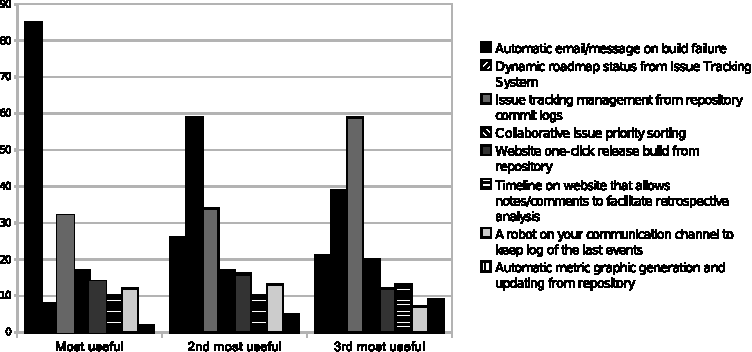
\includegraphics{floss-tools.pdf}
  \caption{FLOSS answers regarding tools usefulness}
  \label{fig:floss-tools}
\end{figure}

Figure \ref{fig:floss-tools} shows the top three choices of most
useful tools within a FLOSS project. Automatic email/message on build
failure was considered the most useful tool by large followed by a
dynamic roadmap status from the issue tracking management system and
issue tracking management from repository commit logs.

\begin{figure}[hbt]
  \centering
  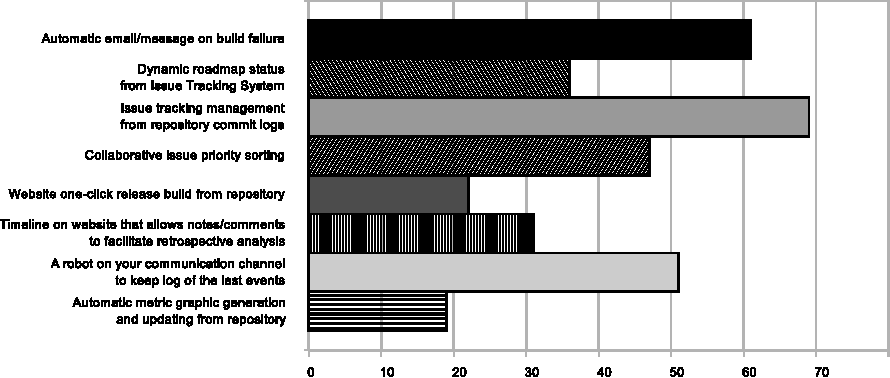
\includegraphics[scale=.8]{floss-existingtools.pdf}
  \caption{Tool participants already use in their FLOSS project}
  \label{fig:floss-existingtools}
\end{figure}

Figure \ref{fig:floss-existingtools} shows that a reasonable amount of
project already have automatic email/message on build failure and
issue tracking management from repository commit logs.

However, we should be aware that Github features an issue tracking
management from repository commits while many other forges don't. And
since Github officially announced the survey, it is probable that many
of their users answered the survey.

\subsection{Individual results from the Agile community}
\label{subsec:agile-results}

The results for the survey directed to the agile community were
collected between 2009/10/01 and 2009/12/01. It received 204 answers
from which 9 were duplicate entries and 34 were invalid due to the use
of incompatible browsers. Such data shows us that about 18\% of the
participants still use browsers incompatible with Javascript
standards. Sensibly more people than in the FLOSS community.

Out of those 161 valid answers, only 28 were from people that never
actually participated in an agile project but considered themselves
as agile practitioners. Another fairly different result from the FLOSS
community. The agile community seems to value ``hands on'' experience
much more than the FLOSS community.

\begin{figure}[htb]
  \begin{minipage}[t]{0.5\linewidth}
    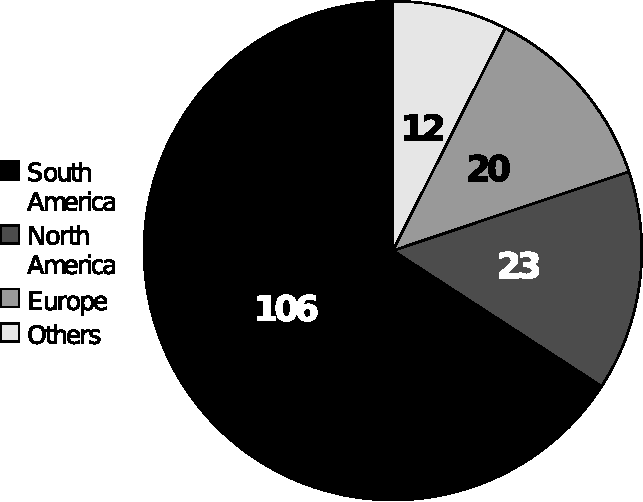
\includegraphics[scale=0.5]{agile-world.pdf}
    \caption{Answers by region of the world}
    \label{fig:agile-world}
  \end{minipage}
  \begin{minipage}[t]{0.5\linewidth}
    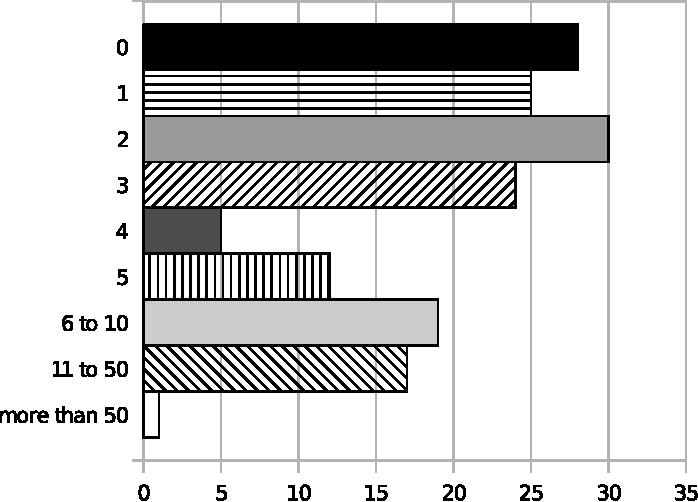
\includegraphics[scale=0.5]{agile-xp.pdf}
    \caption{Number of agile projects experience of the participants}
    \label{fig:agile-xp}
  \end{minipage}
\end{figure}

However it is not a very deep experience since 51\% of the
participants were involved in at most 2 agile projects and only 23\%
had more than 5 agile projects experience. For the rest of the
analysis, participants without any agile experience will not be
counted since they provide little useful data.

For those who had some experience, most still only had a very recent
contact with agile projects. Figure \ref{fig:agile-distributed} shows
that the first experience with agile for most participants only
happened after 2006. We can also see that there is a fairly regular
amount of people with distributed agile experience regardless of the
year of first agile experience.

\begin{figure}[htb]
  \begin{minipage}[t]{0.55\linewidth}
    \centering
    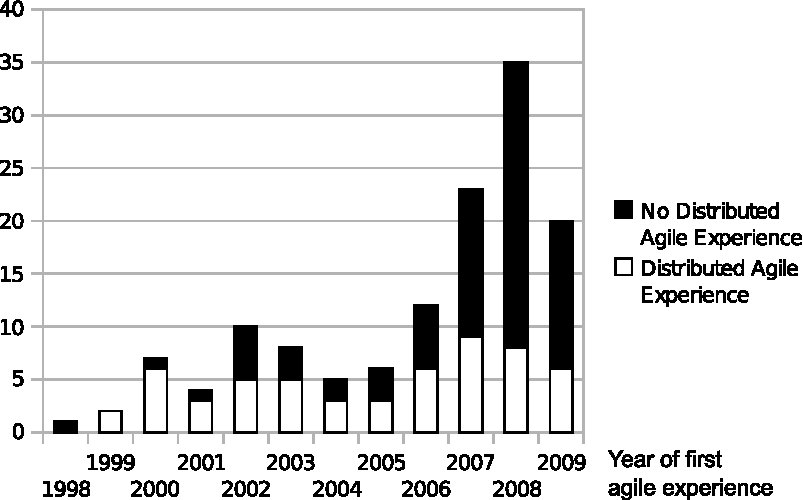
\includegraphics[scale=.45]{agile-distributed.pdf}
    \caption{Distributed agile experience according to the year of the
      first agile experience}
    \label{fig:agile-distributed}
  \end{minipage}
  \begin{minipage}[t]{0.45\linewidth}
    \centering
    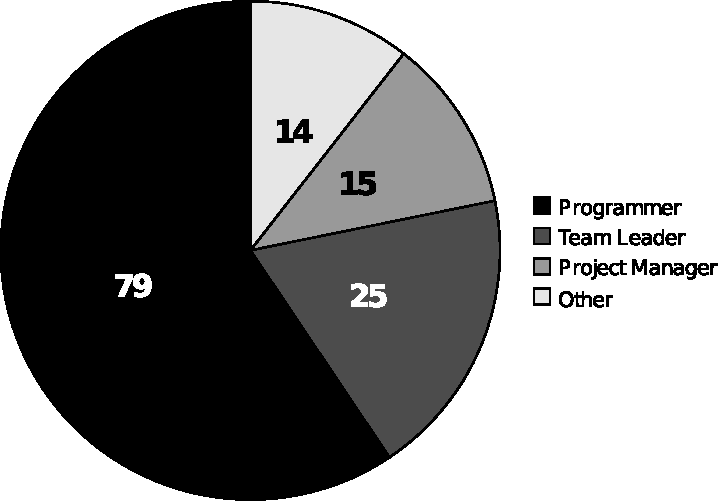
\includegraphics[scale=.45]{agile-roles.pdf}
    \caption{Roles description in the agile community}
    \label{fig:agile-roles}
  \end{minipage}
\end{figure}

Figure \ref{fig:agile-roles} shows that most participants considered
themselves programmers which contrasts with the variety of roles
accumulated in the FLOSS community. Such indication can be justified
by the low hierarchy suggested by some agile books.
% TODO Ref

When it comes to team sizes, smaller teams are obviously
preferred. Figure \ref{fig:agile-teams} shows the distribution of
average team sizes reported by the participants. From such results, it
is clear that a large majority of agile projects involve small teams.

\begin{figure}[htb]
  \begin{minipage}[t]{0.55\linewidth}
    \centering
    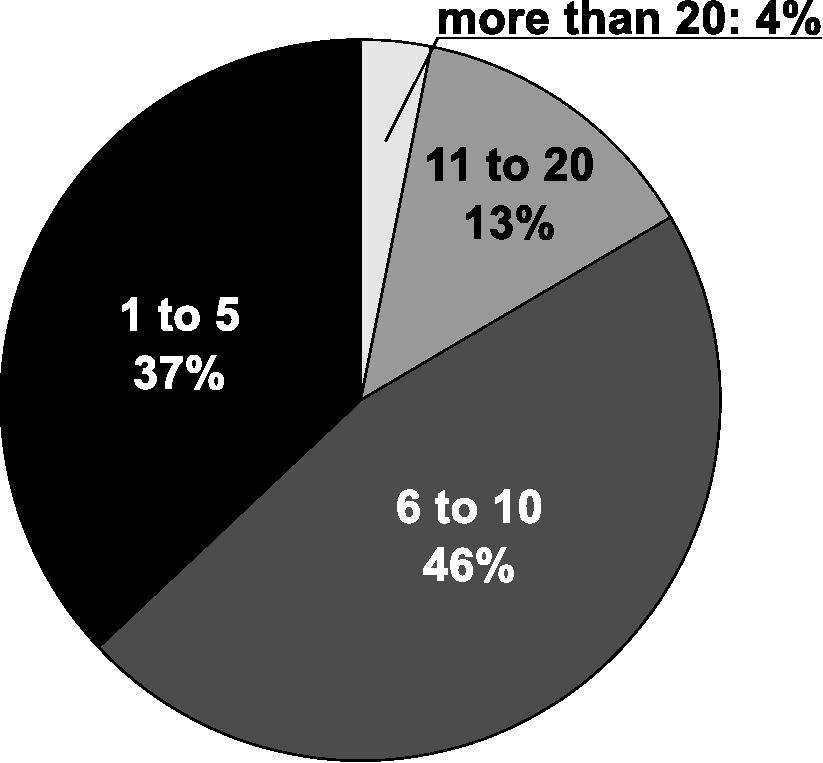
\includegraphics[scale=.3]{agile-teams.pdf}
    \caption{Average agile team sizes}
    \label{fig:agile-teams}
  \end{minipage}
\end{figure}

About 70\% of those teams have face to face communication with their
clients and evaluate the quality of such communication around
67\%. Emails, issue tracking systems and telephones accumulate another
19\% of the teams' communication with their clients with only 54\%,
50\% and 35\% effectiveness respectively. The rest of the channels are
not used enough to provide trustful data.

In distributed environments, the results show that there is no clear
consensus regarding the best communication channel within the
team. There is no clearly most used communication channel nor a
clearly most effective one. However, there is a clearly less effective
one. Emails share a reasonable part of the experiences but are rated
around 31\% effective to communicate between distributed teams.

The ineffectiveness of those communication channel can explain why
56\% of the participants stated that ``discovering what the
users/clients need/want'' is the biggest problem they face on their
agile projects. The second greatest problem is to ``synchronize with
other collaborators to achieve a common goal'' and to ``discover what
is the next task to be done''.

\begin{figure}[hbt]
  \centering
  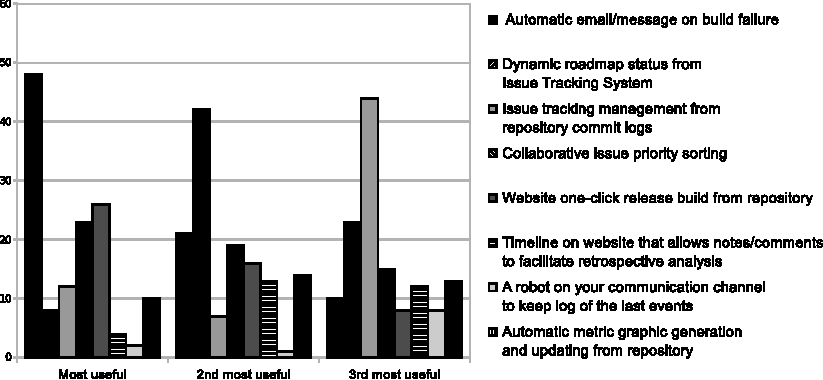
\includegraphics[scale=.9]{agile-tools.pdf}
  \caption{Most useful tools to agile practitioners}
  \label{fig:agile-tools}
\end{figure}

Regarding the useful tools to help agile practitioners, the results
are very similar to the ones listed by FLOSS contributors. The most
useful tools for agile practitioners are exactly the same as for FLOSS
contributors. Messages warning of build failures lead the ranking
followed by dynamic roadmaps and issue tracking management from commit
logs.

Not surprisingly, for the 35\% of the participants that contribute
with FLOSS projects, the problems and tools are the same in that FLOSS
environment. However, they considered their FLOSS projects to be only
``half'' agile. This might indicate that agility and FLOSS development
have the same problems that still need to be solved.

\section{Conclusion}
\label{sec:conclusion}

The results of the survey indicate that the communities are not very
closely related but share common problems and views to solve those
problems. It seems, however, that the most severe issues are not
directly addressed with the suggested tools.

\subsubsection*{Acknowledgments.}

This work was supported by the QualiPSo project \cite{url:qualipso}.

\begin{thebibliography}{5}

\bibitem{report:dempsey1999} Bert J Dempsey and Debra Weiss and Paul
  Jones and Jane Greenberg: A quantitative profile of a community of
  open source Linux developers (1999)

\bibitem{url:agilemanifesto} Kent Beck and Alistair Cockburn and Ward
  Cunningham and Martin Fowler and Ken Schwaber and al.: Manifesto for
  Agile Software Development, http://agilemanifesto.org (2001)

\bibitem{conference:oopsla2007} Dennis Mancl and Steven Fraser and
  William Opdyke: No silver bullet: a retrospective on the essence and
  accidents of software engineering (2007)

\bibitem{brooks1987} Frederick P. Brooks, Jr.: No Silver Bullet:
  Essence and Accidents of Software (1987)

\bibitem{gabriel2005} Ron Goldman and Richard P. Gabriel: Innovation
  Happens Elsewhere: Open Source as Business Strategy (2005)

\bibitem{XP2002} Kent Beck and Cynthia Andres: Extreme Programming
  Explained: Embrace Change, 2nd Edition (2004)

\bibitem{schwaber2004} Ken Schwaber: Agile Project Management with
  Scrum (2004)

\bibitem{cockburn2002} Alistair Cockburn: Agile Software Development
  (2002)

\bibitem{ohno1998} Taiichi Ohno: Toyota Production System: Beyond
  Large-Scale Production (1998)

\bibitem{poppendieck2005} Mary Poppendieck and Tom Poppendieck:
  Introduction to Lean Software Development (2005)

\bibitem{url:fowler2000orig} Martin Fowler: The New Methodology,\\
  http://martinfowler.com/articles/newMethodologyOriginal.html

\bibitem{fogel2005} Karl Fogel: Producing Open Source Software (2005)

\bibitem{url:flossproject} International Institute of Infonomics -
  University of Maastricht: Free/Libre/Open Source Software: Survey
  and Study - Report, http://www.flossproject.org/report/

\bibitem{url:flossdata} International Institute of Infonomics -
  University of Maastricht: Free/Libre/Open Source Software: Survey
  and Study - Report, http://www.flossproject.org/floss1/stats.html

\bibitem{reis2003} Christian Robottom Reis: Caracteriza\c{c}\~{a}o de
  um Processo de Software para Projetos de Software Livre (2003)

\bibitem{raymond1999} Eric S. Raymond: The Cathedral \& the Bazaar:
  Musings on {Linux} and Open Source by an Accidental Revolutionary
  (1999)

\bibitem{crowston2002} Kevin Crowston and Barbara Scozzi: Open source
  software projects as virtual organisations: competency rallying for
  software development (2002)

\bibitem{fitzgerald2000} Joseph Feller and Brian Fitzgerald: A
  framework analysis of the open source software development paradigm
  (2000)

\bibitem{warsta2002} Pekka Abrahamsson and Outi Salo and Jussi
  Ronkainen and Juhani Warsta: Agile software development methods
  (2002)

\bibitem{cockburn2004} Alistair Cockburn: Crystal Clear: A
  Human-Powered Methodology for Small Teams (2004)

  % \bibitem{oram2007} Andy Oram: Why Do People Write Free
  %   Documentation?  Results of a Survey (2007)

  % \bibitem{riehle2007} Dirk Riehle: The Economic Motivation of Open
  %   Source Software: Stakeholder Perspectives (2007)

  % \bibitem{sutherland2007} Jeff Sutherland and Anton Viktorov and
  %   Jack Blount and Nikolai Puntikov: Distributed Scrum: Agile
  %   Project Management with Outsourced Development Teams (2007)

  % \bibitem{maurer2002} Frank Maurer: Supporting Distributed Extreme
  %   Programming (2002)

  % \bibitem{url:beck2008} Kent Beck: Tools for Agility,
  %   http://www.microsoft.com/downloads/details.aspx?FamilyID=ae7e07e8-0872-47c4-b1e7-2c1de7facf96
  %   (2008)

  % \bibitem{nagappan2003} Nachiappan Nagappan and Prashant Baheti and
  %   Laurie Williams and Edward Gehringer and David Stotts: Virtual
  %   Collaboration through Distributed Pair Programming (2003)

  % \bibitem{url:north2006} Dan North: Behaviour Driven Development,
  %   http://dannorth.net/introducing-bdd

  % \bibitem{sato2007} Danilo Sato and Alfredo Goldman and Fabio Kon:
  %   Tracking the Evolution of Object-Oriented Quality Metrics on
  %   Agile Projects (2007)

  % \bibitem{surowiecki2004} J. Surowiecki: The Wisdom of Crowds: Why
  %   the many are smarter than the few and how collective wisdom
  %   shapes business, economies, societies, and nations (2004)

  % \bibitem{tapscott2006} Don Tapscott and Anthony D. Williams:
  %   Wikinomics: How Mass Collaboration Changes Everything (2006)

  % \bibitem{benkler2006} Yochai Benkler: The Wealth of Networks: How
  %   Social Production Transforms Markets and Freedom (2006)

\bibitem{url:qualipso} Qualipso | Trust and Quality in Open Source
  systems, http://www.qualipso.org/
\end{thebibliography}

\appendix
\section{Paper version of the survey to the FLOSS community}
\label{appendix:a}

\begin{enumerate}
\item What country do you live in? \verb=_________________=
  \vspace{10pt}

\item What year where you born? \verb=______= \vspace{10pt}

\item How many FLOSS projects have you already contributed with?

  \verb=( ) 0 ( ) 1 ( ) 2 ( ) 3 ( ) 4 ( ) 5-10 ( ) 11-50 ( ) 51+=
  \vspace{10pt}

\item What is the name of the FLOSS project you mostly contribute (or
  contributed) with? \verb= ______________= \vspace{10pt}

\item In which year was your first contribution to that project?
  \verb=______= \vspace{10pt}

\item What is (or was) your main role in that project?
  \begin{itemize}
    \begin{minipage}[t]{0.5\linewidth}
    \item[( ) ] Maintainer
    \item[( ) ] Commiter
    \item[( ) ] Programmer
    \item[( ) ] Tester
    \end{minipage}
    \begin{minipage}[t]{0.5\linewidth}
    \item[( ) ] Documentation writer
    \item[( ) ] Bug reporter/Feature requester
    \item[( ) ] User
    \item[( ) ] Other: \verb=_________________=
    \end{minipage}
  \end{itemize}
  \vspace{10pt}

\item Do (Did) you receive any income from your FLOSS contributions?
  \verb=( ) Yes ( ) No= \vspace{10pt}

\item If you do (did), is (was) this your main income?
  \verb=( ) Yes ( ) No= \vspace{10pt}

\item If you do (did) not receive any income from your contributions
  or if those contributions were not your main income), is (was) your
  main income related to IT?  \verb=( ) Yes ( ) No= \vspace{10pt}

\item How many people work (or worked) with you on your main FLOSS
  project?  \verb=( ) 0 ( ) 1-5 ( ) 6-10 ( ) 11-50 ( ) 51+=
  \vspace{10pt}

\item What is (or was) your main communication channel with your team
  of that FLOSS project?
  \begin{itemize}
    \begin{minipage}[t]{0.5\linewidth}
    \item[( ) ] Face to face
    \item[( ) ] Website
    \item[( ) ] Mailing list
    \item[( ) ] Issue tracker (Trac, Bugzilla, etc.)
    \item[( ) ] Internet Relay Chat (IRC)
    \end{minipage}
    \begin{minipage}[t]{0.5\linewidth}
    \item[( ) ] Instant Message (Jabber, ICQ, etc.)
    \item[( ) ] Email
    \item[( ) ] VoIP (Skype, Ekiga, iChat, etc.)
    \item[( ) ] None
    \item[( ) ] Other: \verb=_____________=
    \end{minipage}
  \end{itemize}
  \vspace{10pt}

\item How would you evaluate the quality of your communication with
  that team?

  Extremely poor \verb=---------------------------------------=
  Perfect \vspace{10pt}

\item What is (or was) your main communication channel with the users
  of that FLOSS project?
  \begin{itemize}
    \begin{minipage}[t]{0.5\linewidth}
    \item[( ) ] Face to face
    \item[( ) ] Website
    \item[( ) ] Mailing list
    \item[( ) ] Issue tracker (Trac, Bugzilla, etc.)
    \item[( ) ] Internet Relay Chat (IRC)
    \end{minipage}
    \begin{minipage}[t]{0.5\linewidth}
    \item[( ) ] Instant Message (Jabber, ICQ, etc.)
    \item[( ) ] Email
    \item[( ) ] VoIP (Skype, Ekiga, iChat, etc.)
    \item[( ) ] None
    \item[( ) ] Other: \verb=_____________=
    \end{minipage}
  \end{itemize}
  \vspace{10pt}

\item How would you evaluate the quality of your communication with
  the users?

  Extremely poor \verb=---------------------------------------=
  Perfect \vspace{10pt}

\item How much effort do (or did) you spend to keep the project's
  information updated?

  Very little \verb=---------------------------------------= Huge
  \vspace{10pt}

\item Which of the following tools does (or did) your project already
  use?
  \begin{itemize}
  \item[[ ] ] Automatic email/message on build failure
  \item[[ ] ] Dynamic roadmap status from Issue Tracking System
  \item[[ ] ] Issue tracking management from repository commit logs
  \item[[ ] ] Website one-click release build from repository
  \item[[ ] ] Automatic metric graphic generation and updating from
    repository
  \item[[ ] ] Collaborative issue priority sorting
  \item[[ ] ] Timeline on website that allows notes/comments to
    facilitate retrospective analysis
  \item[[ ] ] A robot on your communication channel to keep log of the
    last events
  \end{itemize}
  \vspace{10pt}

\item Sort the tools from the most useful (first) to the less useful
  (last).
  \begin{itemize}
  \item[( ) ] Automatic email/message on build failure
  \item[( ) ] Dynamic roadmap status from Issue Tracking System
  \item[( ) ] Issue tracking management from repository commit logs
  \item[( ) ] Website one-click release build from repository
  \item[( ) ] Automatic metric graphic generation and updating from
    repository
  \item[( ) ] Collaborative issue priority sorting
  \item[( ) ] Timeline on website that allows notes/comments to
    facilitate retrospective analysis
  \item[( ) ] A robot on your communication channel to keep log of the
    last events
  \end{itemize}
\end{enumerate}

\section{Paper version of the survey to the agile community}
\label{appendix:b}

\begin{enumerate}
\item What country do you live in? \verb=_________________=
  \vspace{10pt}

\item What year where you born? \verb=______= \vspace{10pt}

\item How many projects you would consider agile have you been on?

  \verb=( ) 0 ( ) 1 ( ) 2 ( ) 3 ( ) 4 ( ) 5-10 ( ) 11-50 ( ) 51+=
  \vspace{10pt}

\item In which year was the first Agile project you participated?
  \verb=______= \vspace{10pt}

\item What is (or was) your main role in that project?
  \begin{itemize}
    \begin{minipage}[t]{0.5\linewidth}
    \item[( ) ] Project manager
    \item[( ) ] Team leader
    \item[( ) ] Programmer
    \item[( ) ] Quality Analyst
    \end{minipage}
    \begin{minipage}[t]{0.5\linewidth}
    \item[( ) ] Tester
    \item[( ) ] Tracker
    \item[( ) ] Documenter
    \item[( ) ] Other: \verb=_________________=
    \end{minipage}
  \end{itemize}
  \vspace{10pt}

\item What is (or was) the average number of people in the agile
  projects you worked?
  \verb=( ) 1-5 ( ) 6-10 ( ) 11-20 ( ) 21-50 ( ) 51-100 ( )100+=
  \vspace{10pt}

\item What is (or was) your main communication channel with the
  clients of that project?
  \begin{itemize}
    \begin{minipage}[t]{0.5\linewidth}
    \item[( ) ] Face to face
    \item[( ) ] Website
    \item[( ) ] Mailing list
    \item[( ) ] Issue tracker (Trac, Bugzilla, etc.)
    \item[( ) ] Internet Relay Chat (IRC)
    \item[( ) ] Other: \verb=_____________=
    \end{minipage}
    \begin{minipage}[t]{0.5\linewidth}
    \item[( ) ] Instant Message (Jabber, ICQ, etc.)
    \item[( ) ] Email
    \item[( ) ] Telephone
    \item[( ) ] VoIP (Skype, Ekiga, iChat, etc.)
    \item[( ) ] None
    \end{minipage}
  \end{itemize}
  \vspace{10pt}

\item How would you evaluate the quality of your communication with
  the clients?

  Extremely poor \verb=---------------------------------------=
  Perfect \vspace{10pt}

\item Have you ever been on a distributed agile project?
  \verb=( ) Yes ( ) No= \vspace{10pt}

\item If yes, what is (or was) your main communication channel within
  that distributed team?
  \begin{itemize}
    \begin{minipage}[t]{0.5\linewidth}
    \item[( ) ] Face to face
    \item[( ) ] Website
    \item[( ) ] Mailing list
    \item[( ) ] Issue tracker (Trac, Bugzilla, etc.)
    \item[( ) ] Internet Relay Chat (IRC)
    \item[( ) ] Other: \verb=_____________=
    \end{minipage}
    \begin{minipage}[t]{0.5\linewidth}
    \item[( ) ] Instant Message (Jabber, ICQ, etc.)
    \item[( ) ] Email
    \item[( ) ] Telephone
    \item[( ) ] VoIP (Skype, Ekiga, iChat, etc.)
    \item[( ) ] None
    \end{minipage}
  \end{itemize}
  \vspace{10pt}

\item If you had distributed agile experience, how would you evaluate
  the quality of your communication with that team?

  Extremely poor \verb=---------------------------------------=
  Perfect \vspace{10pt}

\item For some of the common problems encountered by agile teams
  listed below, sort the 3 most critical problems in the agile
  environments you worked on.
  \begin{itemize}
  \item[[ ] ] Discover what the users/clients need/want
  \item[[ ] ] Discover what is the next task to be done
  \item[[ ] ] Understand how the project works from a technical point
    of view
  \item[[ ] ] Discover the current project status
  \item[[ ] ] Integrate the source code to the main repository
  \item[[ ] ] Keep the information about the project updated in its
    main communication channel
  \item[[ ] ] Evaluate the work done to identify improvement points
  \item[[ ] ] Synchronize with other collaborators to achieve a common
    goal
  \end{itemize}
  \vspace{10pt}

\item Sort the 3 tools that would most help you in a distributed agile
  environment.
  \begin{itemize}
  \item[[ ] ] Automatic email/message on build failure
  \item[[ ] ] Dynamic roadmap status from Issue Tracking System
  \item[[ ] ] Issue tracking management from repository commit logs
  \item[[ ] ] Website one-click release build from repository
  \item[[ ] ] Automatic metric graphic generation and updating from
    repository
  \item[[ ] ] Collaborative issue priority sorting
  \item[[ ] ] Timeline on website that allows notes/comments to
    facilitate retrospective analysis
  \item[[ ] ] A robot on your communication channel to keep log of the
    last events
  \end{itemize}
\vspace{10pt}

\item Have you ever contributed to Free, Libre, Open Source Software
  (FLOSS)?  \verb=( ) Yes ( ) No= \vspace{10pt}

\item How would you evaluate the agile level of your FLOSS project?

  Anti agile \verb=---------------------------------------= Very agile
  \vspace{10pt}

\item For some of the common problems encountered by agile teams
  listed below, sort the 3 most critical problems in the FLOSS
  projects you worked on.
  \begin{itemize}
  \item[[ ] ] Discover what the users/clients need/want
  \item[[ ] ] Discover what is the next task to be done
  \item[[ ] ] Understand how the project works from a technical point
    of view
  \item[[ ] ] Discover the current project status
  \item[[ ] ] Integrate the source code to the main repository
  \item[[ ] ] Keep the information about the project updated in its
    main communication channel
  \item[[ ] ] Evaluate the work done to identify improvement points
  \item[[ ] ] Synchronize with other collaborators to achieve a common
    goal
  \end{itemize}
  \vspace{10pt}

\item Sort the 3 tools that would most help you in that FLOSS
  environment.
  \begin{itemize}
  \item[[ ] ] Automatic email/message on build failure
  \item[[ ] ] Dynamic roadmap status from Issue Tracking System
  \item[[ ] ] Issue tracking management from repository commit logs
  \item[[ ] ] Website one-click release build from repository
  \item[[ ] ] Automatic metric graphic generation and updating from
    repository
  \item[[ ] ] Collaborative issue priority sorting
  \item[[ ] ] Timeline on website that allows notes/comments to
    facilitate retrospective analysis
  \item[[ ] ] A robot on your communication channel to keep log of the
    last events
  \end{itemize}
\end{enumerate}
\end{document}
